\documentclass[9pt]{article}

%For better code
\usepackage{verbatim} 			%Allows begin{comment} and end{comment}
%Also allows for the "verbatim" package
\pagestyle{plain} %includes page numbers
\usepackage[margin=0.70in]{geometry} %included to change page margins
\usepackage[pdftex]{graphicx} %included to insert a graph
\usepackage{grffile} %allows to use spaces in file names when using pdflatex
%\usepackage{caption} %included to include a caption over the graph

\usepackage[section]{placeins} %to keep graphs and tables in the very section to which they belong
\usepackage{pdflscape} %to include the landscape environment
\usepackage{setspace} %to allow for doubleline spacing, etc
\usepackage{natbib} % for fancy bibliographies
\usepackage{amsmath}	 % Packages for Mathematics
\usepackage{amssymb}
\usepackage{amsthm}
\usepackage{hyperref}

%For the tables and graphs
\usepackage{booktabs}		%For different style lines
\usepackage{calc}			%Necessary for the text wrapping command on tables.
\usepackage{array}			%For better tables (wrapping text in cells)
\usepackage{rotating}		%For rotated tables
\usepackage{longtable}		%Allows tables to extend past one page
\usepackage{float} 			%Allows to suppress floating of tables
\usepackage{tabularx}		%Provides more alignment options, and specifying table width
\usepackage{placeins}		%For floatbarrier
%\usepackage[lmargin=2cm, rmargin=2cm,tmargin=2.4cm,bmargin=2cm]{geometry}
\onehalfspacing
\usepackage{supertabular}


\usepackage{multirow}
\usepackage{array}
\usepackage{latexsym}
\usepackage{ctable}
\usepackage{dcolumn}
\def\sym#1{\ifmmode^{#1}\else\(^{#1}\)\fi}
\newcommand{\specialcell}[2][c]{
	\begin{tabular}[#1]{@{}c@{}}#2\end{tabular}}
\setlength\parindent{0em}


\usepackage{dcolumn} % to be able to center on the decimal, and add in stata: alignment(D{.}{.}{-1})
\newcolumntype{C}[1]{>{\centering\arraybackslash\hspace{0pt}}p{#1}}
\usepackage{enumitem}
\usepackage{caption}
\usepackage{subcaption}
\usepackage[english]{babel} %%% 'french', 'german', 'spanish', 'danish', etc.
\usepackage{amssymb}
\usepackage{amsmath}
%\usepackage{txfonts} % commented out by Carolyn to resume regular font
\usepackage{mathdots}
%\usepackage[classicReIm]{kpfonts} % commented out by Carolyn to resume regular font


\usepackage{makecell}

\renewcommand\theadalign{cb}
\renewcommand\theadfont{\bfseries}
\renewcommand\theadgape{\Gape[4pt]}
\renewcommand\cellgape{\Gape[4pt]}

\onehalfspacing
\setlength\parindent{15pt}
%begin the document
\usepackage{natbib}


\usepackage{array}
\usepackage{xcolor}
\hypersetup{
	colorlinks   = true, %Colours links instead of ugly boxes
	urlcolor     = red, %Colour for external hyperlinks
	linkcolor    = blue, %Colour of internal links
	citecolor   = blue %Colour of citations
}

\usepackage{adjustbox}
\usepackage{threeparttable}
\usepackage{soul}

\author{Hongdi Zhao}
\title{Summary Statistics}
\date{\today}


\begin{document}
	\maketitle
	\tableofcontents
	

\newpage
\section{Balance Table}

\begin{center} \footnotesize  
\tablefirsthead{ \cmidrule{2-4} \\  & \parbox[c]{2.5cm}{ \centering \textbf{Control} \\ \vspace{2mm} Mean [SD] } & \parbox[c]{2.5cm}{ \centering \textbf{Treatment} \\ \vspace{2mm} Mean diff. (SE)}  & \parbox[c]{2.5cm}{ \centering Nr. Obs} \\ \\ & [1] & [2] & [3] \\ \midrule } 
\tablehead{  \multicolumn{4}{r}{\small\sl \ldots continued from previous page}\\ \cmidrule{2-4}  \\  & \parbox[c]{2.5cm}{ \centering \textbf{Control} \\ \vspace{2mm} Mean [SD] } &  \parbox[c]{2.5cm}{ \centering \textbf{Treatment} \\ \vspace{2mm} Mean diff. (SE)}  & \parbox[c]{2.5cm}{ \centering Nr. Obs} \\ \\ & [1] & [2] & [3]  \\ \midrule }
\tabletail{\midrule \multicolumn{4}{r}{\small\sl continued to next page\ldots}\\} \tablelasttail{\midrule \midrule} 
\topcaption{Baseline Balance Checks}
\renewcommand{\arraystretch}{0.85}
\begin{supertabular}{l C{2.5cm} C{2.5cm} C{2.5cm}}
\multicolumn{4}{l}{\textbf{Panel A: Demographics}}\\
\hspace{0.4cm} Household Head is Male &    0.73&   -0.02&    4100\\
 &[   0.44 ]& (   0.02 ) & \\
\hspace{0.4cm} Years of Education of Household Head &    7.47&    0.06&    4100\\
 &[   4.72 ]& (   0.22 ) & \\
\hspace{0.4cm} Number of Household Members &    4.60&   -0.14$^{\star \star}$&    4100\\
 &[   1.91 ]& (   0.07 ) & \\
\hspace{0.4cm} Most Backward Caste &    0.31&    0.05&    4087\\
 &[   0.46 ]& (   0.04 ) & \\
\hspace{0.4cm} Scheduled Caste and Tribe &    0.25&   -0.00&    4087\\
 &[   0.43 ]& (   0.03 ) & \\
\hspace{0.4cm} Household Own Land &    0.55&   -0.00&    4091\\
 &[   0.50 ]& (   0.04 ) & \\
\hspace{0.4cm} Female Respondent Age &   30.41&   -0.12&    4058\\
 &[  15.62 ]& (   0.63 ) & \\
\hspace{0.4cm} Female Respondent Years of Education &    6.12&   -0.09&    4058\\
 &[   5.28 ]& (   0.26 ) & \\
\multicolumn{4}{l}{}\\
\multicolumn{4}{l}{\textbf{Panel B: Income \& Consumption Outcomes}}\\
\hspace{0.4cm} Tot HH Consumption (30-day), top-coded & 3347.62& -113.63&    4096\\
 &[2465.07 ]& ( 168.96 ) & \\
\hspace{0.4cm} Tot HH Income (30-day), top-coded & 6446.46&   74.01&    2743\\
 &[7582.34 ]& ( 543.17 ) & \\
\hspace{0.4cm} Below Poverty Line (using Consumption) &    0.83&    0.02&    4095\\
 &[   0.38 ]& (   0.02 ) & \\
\hspace{0.4cm} Below Poverty Line (using Income) &    0.53&   -0.00&    2741\\
 &[   0.50 ]& (   0.03 ) & \\
\multicolumn{4}{l}{}\\
\multicolumn{4}{l}{\textbf{Panel C: Borrowing \& Saving \& Insurance Outcomes}}\\
\hspace{0.4cm} Household has Outstanding Formal Loan(s) &    0.61&    0.00&    4057\\
 &[   0.49 ]& (   0.02 ) & \\
\hspace{0.4cm} Household has Outstanding Informal Loan(s) &    0.72&   -0.01&    4057\\
 &[   0.45 ]& (   0.02 ) & \\
\hspace{0.4cm} Household Has Active Insurance &    0.80&    0.01&    4091\\
 &[   0.40 ]& (   0.02 ) & \\
\hspace{0.4cm} Tot. Savings Amt (Rs) & 4409.36&  243.42&    3988\\
 &[9370.65 ]& ( 405.88 ) & \\
\hspace{0.4cm} Informal Share of Tot. Outstnd Ratio &    0.48&   -0.01&    3810\\
 &[   0.43 ]& (   0.02 ) & \\
\multicolumn{4}{l}{}\\ \end{supertabular}
\footnotesize \begin{tabular}{p{17cm}} 
\textbf{Note :} ***(**)(*) indicates significance at the 1\%(5\%)(10\%) level. Column [1] reports control group means, with standard deviations in parentheses. Column [2] reports the OLS coefficient estimates associated with regressing each outcome on a dummy indicating treatment. Pair fixed effects are included. Standard errors are clustered at the service area level. Column [3] reports the number of observations. All Rs. values are top-coded three standard deviations from the mean, unless otherwise specified. 
 \end{tabular} \end{center}


\newpage
\section{Regression}
\begin{table}[H]
\centering
\caption{Impact
on
Income
and
Borrowing}
\label{"incpov"}
\small
\begin{tabular}{l
C{1.7cm}
C{1.7cm}
C{1.9cm}
C{1.9cm}}
\cmidrule{2-5}
\\
&
Log
Tot
HH
Income
(Last
30
days)
&
Log
Tot
HH
Consumption
(Last
30
days)
&
Total
Formal
Borrowed
Loan
(24
month)
&
Total
Informal
Borrowed
Loan
(24
month)
\\
\midrule
\multicolumn{5}{l}{\textit{\textbf{Panel
A:
Without
Controls}}}\\
\midrule
                    &\multicolumn{1}{c}{(1)}         &\multicolumn{1}{c}{(2)}         &\multicolumn{1}{c}{(3)}         &\multicolumn{1}{c}{(4)}         \\
\midrule
Treated             &        0.10         &       -0.00         &     7033.18         &    -4340.50         \\
                    &      (0.05)\sym{*}  &      (0.02)         &   (2259.99)\sym{***}&   (1668.50)\sym{**} \\
\midrule
Control Dep Var Mean&        8.16         &        8.19         &    56423.12         &    39800.40         \\
\textit{N}          &        4183         &        4184         &        4158         &        4158         \\

 \\ \midrule \multicolumn{5}{l}{\textit{\textbf{Panel B: With Control}}} \\ \midrule 
                    &\multicolumn{1}{c}{(1)}         &\multicolumn{1}{c}{(2)}         &\multicolumn{1}{c}{(3)}         &\multicolumn{1}{c}{(4)}         \\
\midrule
Treated             &        0.13         &        0.02         &     7453.17         &    -3992.95         \\
                    &      (0.05)\sym{**} &      (0.02)         &   (2189.91)\sym{***}&   (1644.01)\sym{**} \\
\midrule
Control Dep Var Mean&        8.16         &        8.19         &    56423.12         &    39800.40         \\
\textit{N}          &        4183         &        4184         &        4158         &        4158         \\
 \bottomrule \end{tabular} \footnotesize \begin{tabular}{p{13cm}}{\textbf{Note:} ***, **, * indicates significance at the 1\%, 5\%,                                  and 10\% level respectively. OLS estimates (standard errors)                                  are reported from regressing each dependent variable on a                                  dummy indicating whether the household resides in a treated                                  service area. } \end{tabular} \end{table}



\newpage
\section{Appendix}
\subsection{Other Summary}
\begin{table}[htbp]\centering
\caption{Consent to Survey\label{tab1-consent}}
\begin{tabular}{l*{6}{c}}
\toprule
                    & Not Consent&   Consented&   [Complete&  Ineligible&Eligible for Revisit&Revoke Consent Midway]\\
\midrule
23-02-2020          &           3&         124&         123&           0&           0&           1\\
24-02-2020          &           5&         133&         132&           0&           0&           1\\
25-02-2020          &           2&         122&         119&           2&           0&           1\\
26-02-2020          &           0&          94&          92&           2&           0&           0\\
Total               &          10&         473&         466&           4&           0&           3\\
\bottomrule
\end{tabular}
\end{table}

\begin{table}[htbp]\centering
\caption{Completed Survey Status by Village\label{tab1-progress-byvillage}}
\begin{tabular}{l*{5}{c}}
\toprule
                    &    Complete&  Ineligible&Eligible for Revisit&Not Consent/Revoke Consent Midway&       Total\\
\midrule
Gehri Bara Singh    &          65&         213&          16&           5&         299\\
Gurusar             &          63&         202&          26&           6&         297\\
Nehianwala          &         224&        1004&          93&          44&        1365\\
Phullo Mithi        &         114&         590&          45&           0&         749\\
Total               &         466&        2009&         180&          55&        2710\\
\bottomrule
\end{tabular}
\end{table}



\subsection{GPS Coordinates}
\begin{figure}[H]
	\centering
	\caption{Check GPS Coordinates}
	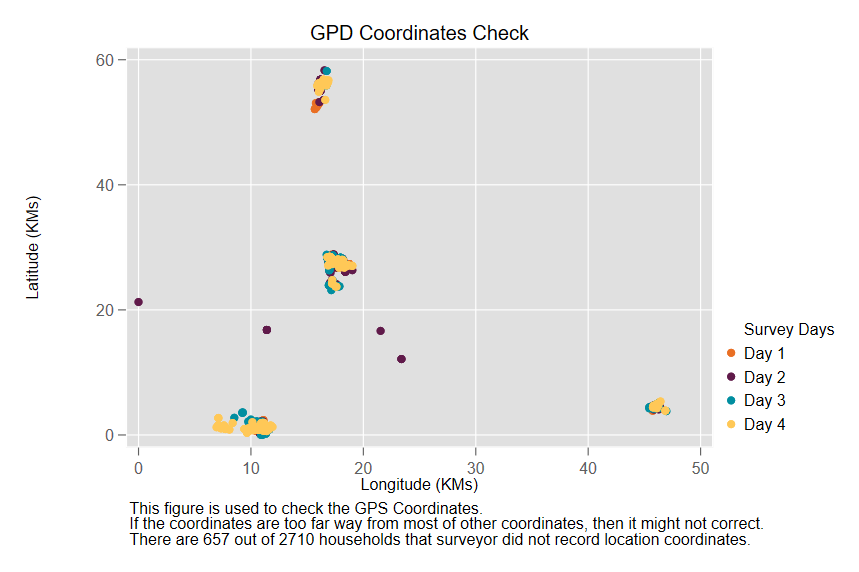
\includegraphics[scale=0.50]{../4_figures/gps_check_pilot.png}
\end{figure}



\begin{figure}[H]
	\centering
	\caption{Check GPS Coordinates - Gehri Bara Singh}
	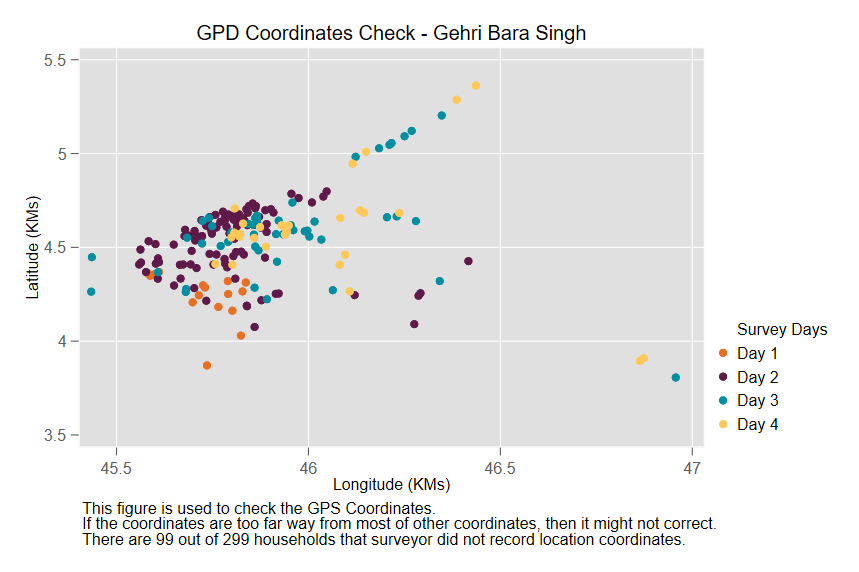
\includegraphics[scale=0.50]{../4_figures/gps_check_pilot_1.png}
\end{figure}



\begin{figure}[H]
	\centering
	\caption{Check GPS Coordinates - Gurusar}
	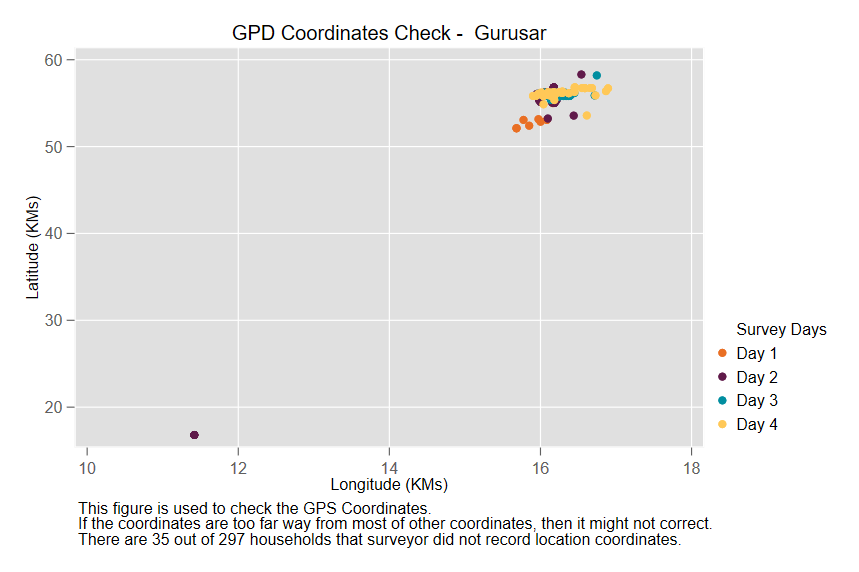
\includegraphics[scale=0.50]{../4_figures/gps_check_pilot_2.png}
\end{figure}



\end{document}
